The message signal is available in 
\begin{lstlisting}
fm/msg/codes/Sound_Noise.wav
\end{lstlisting}
\begin{enumerate}[label=\arabic*.,ref=\thesection.\theenumi]
\numberwithin{equation}{enumi}
\item Plot the spectrum of the message signal.\\
\solution The spectrum of input audio signal is plotted below\\
\begin{figure}[h]
    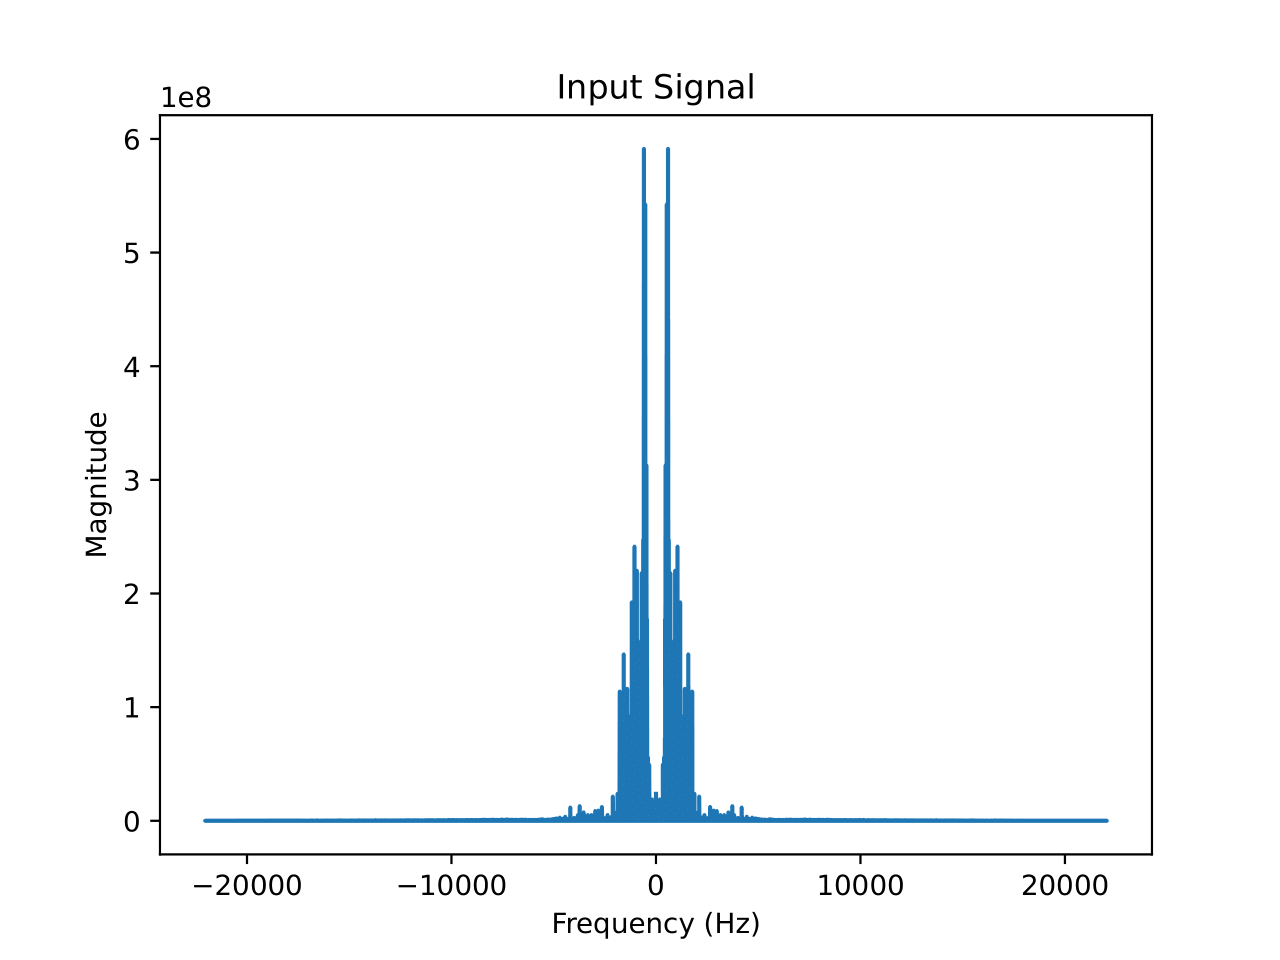
\includegraphics[scale=0.55]{fm/msg/inputs-1.png}
\end{figure}
\\
To plot the spectrum of the message signal, we need to compute the Fourier Transform of the message signal, which will give us the frequency domain representation of the signal.
\begin{equation}
M_k = \sum_{n=0}^{N-1} m(n) e^{-j2\pi kn/N}, \quad k=0,1,\dots,N-1
\end{equation}
\\
The code to plot the spectrum of the message signal is given below
\begin{lstlisting}
fm/msg/codes/FFTmsg.py
\end{lstlisting}
\item Find the bandwidth of the message signal.\\
\solution The bandwidth can be calculated mathematically using the following formula:
\begin{align*}
B=mask_{maxi}-mask_{min}
\end{align*}
where $mask_{maxi}$ and $mask_{min} $ are themaximum amd minimum frequency bounds of the range  respectively.\\
Analyzes the audio signal and plots its magnitude spectrum. The bandwidth of the audio signal is  calculated using power spectral density. Obtain the bandwidth of the audio as 2 khz using below code
\begin{center}
\fcolorbox{red}{white}{\parbox{7.5cm}
{\href{https://github.com/KrishnaYadati/signal-processing/tree/main/fm/codes/input.py}
{/codes/input.py}}}
\end{center}
\end{enumerate}
